\documentclass[12pt,a4paper]{report}

\usepackage[utf8]{inputenc}
\usepackage{graphicx}
\usepackage{hyperref}
\usepackage{amsmath}
\usepackage{booktabs}
\usepackage{geometry}
\usepackage{hyperref}
\usepackage{setspace}
\usepackage{titlesec}
\usepackage{titling}
\usepackage{listings}
\usepackage{xcolor}
\usepackage{natbib}
%\usepackage[toc]{glossaries}
\usepackage[acronym]{glossaries}
\usepackage{fancyhdr}
\pagestyle{fancy}
\fancyhf{}
\fancyhead[R]{\makebox[\textwidth][r]{Enhancing Fraud Detection in Bank Accounts}}
\fancyfoot[C]{\thepage}
\renewcommand{\headrulewidth}{0pt}


\lstset{
    basicstyle=\ttfamily\footnotesize,
    keywordstyle=\color{blue},
    commentstyle=\color{gray},
    stringstyle=\color{red},
    showstringspaces=false,
    breaklines=true,
    frame=single,
    captionpos=b,
    aboveskip=10pt,
    belowskip=10pt
}

\geometry{a4paper, top=2cm, bottom=2cm, left=2cm, right=2cm}
\setstretch{1.5}

% Chapter, section, and subsection formatting
\titleformat{\chapter}[block]{\normalfont\huge\bfseries}{\thechapter}{1em}{}
\titleformat{\section}[block]{\normalfont\Large\bfseries}{\thesection}{1em}{}
\titleformat{\subsection}[block]{\normalfont\large\bfseries}{\thesubsection}{1em}{}
\titlespacing*{\chapter}{0pt}{0pt}{12pt}
\titlespacing*{\section}{0pt}{12pt}{6pt}
\titlespacing*{\subsection}{0pt}{12pt}{6pt}

% Footnotes font size
\makeatletter
\renewcommand\footnoterule{%
    \kern-3\p@
    \hrule\@width\columnwidth
    \kern2.6\p@}
\renewcommand\@makefntext[1]{%
    \noindent\makebox[1.8em][r]{\@makefnmark}#1}
\renewcommand{\footnotesize}{\fontsize{10pt}{12pt}\selectfont}
\makeatother

% title page
\renewcommand{\maketitle}{
    \begin{titlepage}
       \noindent
        \vspace*{1cm}
        \begin{center}
            % Centered logo
            
\includegraphics[width=0.5\textwidth]{iu_Logo_EN_black_RGB_horizontal.jpg}\\[0.5cm]
    
            \textbf{\fontsize{14pt}{16pt}\selectfont Master Thesis}
            \vspace{1.5cm}
    
            \textbf{\fontsize{14pt}{16pt}\selectfont IU University of Applied Sciences}
            \vspace{0.5cm}
    
            \textbf{\fontsize{14pt}{16pt}\selectfont Study programme: Data Science}
            \vspace{2.0cm}
    
            \textbf{\fontsize{14pt}{16pt}\selectfont Enhancing Fraud Detection in Bank Accounts Through Machine Learning: A Case Study Using the BAF Suite}
            
            \vspace{2.0cm}
            \textbf{\fontsize{14pt}{16pt}\selectfont Volkan Karaarslan}\\
            \vspace{0.5cm}
            \textbf{\fontsize{14pt}{16pt}\selectfont Enrolment number: 92114860}\\
            
            \vspace{0.5cm}
            
            \textbf{\fontsize{14pt}{16pt}\selectfont Bernhard-Letterhaus Str. 25}\\
            \vspace{0.5cm}
            \textbf{\fontsize{14pt}{16pt}\selectfont 41466 Neuss}
            
        \end{center}
        
        % Add lines at the bottom of the title page, beginning from left margin
        \vspace*{\fill}
        \noindent
        \textbf{\fontsize{14pt}{16pt}\selectfont Supervisor: Prof. Robert Graf}\\
        \textbf{\fontsize{14pt}{16pt}\selectfont Date of submission: 1st August 2024}
    \end{titlepage}
}

\makeglossaries
\newacronym{adasyn}{ADASYN}{Adaptive Synthetic Sampling Approach for Imbalanced Learning}
\newacronym{ai}{AI}{Artificial Intelligence}
\newacronym{auc}{AUC}{Area Under the Curve}
\newacronym{baf}{BAF}{Bank Account Fraud}
\newacronym{cart}{CART}{Classification and Regression Trees}
\newacronym{crispdm}{CRISP-DM}{Cross-Industry Standard Process for Data Mining}
\newacronym{ctgan}{CTGAN}{Conditional Tabular Generative Adversarial Network}
\newacronym{dl}{DL}{Deep Learning}
\newacronym{dm}{DM}{Data Mining}
\newacronym{drl}{DRL}{Deep Reinforcement Learning}
\newacronym{eda}{EDA}{Exploratory Data Analysis}
\newacronym{gan}{GAN}{Generative Adversarial Network}
\newacronym{iu}{IU}{Interpretation Unit}
\newacronym{mb}{MB}{Megabyte}
\newacronym{ml}{ML}{Machine Learning}
\newacronym{nc}{NC}{Normalized Cut}
\newacronym{ndcg}{NDCG}{Normalized Discounted Cumulative Gain}
\newacronym{ndcg@k}{NDCG@k}{Normalized Discounted Cumulative Gain at the Position k}
\newacronym{nn}{NN}{Neural Networks}
\newacronym{os}{OS}{Operating System}
\newacronym{rdqn}{RDQN}{Reinforcement Deep Q-Network}
\newacronym{roc}{ROC}{Receiver Operating Characteristic}
\newacronym{rus}{RUS}{Random Under Sampling}
\newacronym{smote}{SMOTE}{Synthetic Minority Over-sampling Technique}
\newacronym{smotenc}{SMOTE-NC}{Synthetic Minority Over-sampling Technique for Nominal and Continuous}
\newacronym{zip}{ZIP}{Zone Improvement Plan}

\begin{document}

\maketitle


\begin{abstract}
This thesis explores the application of machine learning techniques in detecting fraudulent activities within bank accounts using the \acrshort{baf} \href{https://www.kaggle.com/datasets/sgpjesus/bank-account-fraud-dataset-neurips-2022/code}{Suite}. It aims to develop and evaluate a machine learning model for fraud detection, thereby improving detection accuracy, increasing working efficiency, and mitigating social inequities caused by biased predictions.
\end{abstract}

\printglossary[type=\acronymtype, title=Abbreviations]
\pagenumbering{gobble}

%\printglossary
\clearpage

\tableofcontents

\pagenumbering{gobble}


\clearpage


\chapter{Introduction}

\pagenumbering{arabic}

\section{Background}
Fraud detection has become increasingly critical in the financial sector due to the significant rise in fraudulent activities. Banks and financial institutions are particularly vulnerable to fraud, which can result in substantial financial losses and damage to reputation. Traditionally, fraud detection systems relied on rule-based methods, which, although effective to some extent, often fail to adapt to new and sophisticated fraudulent techniques.\\

With the advent of machine learning, there has been a paradigm shift in the approach to fraud detection. Machine learning models, with their ability to learn from vast amounts of data and identify patterns, offer a promising solution to detecting fraudulent activities (\citealp[p.4]{bao2020detecting}). The \acrshort{baf} \href{https://www.kaggle.com/datasets/sgpjesus/bank-account-fraud-dataset-neurips-2022/code}{Suite} is a synthetic bank account data set that may be used to test fraud detection capabilities (\citealp{jesus2022turning}). However, the implementation of these models must also consider fairness, ensuring that the models do not perpetuate or exacerbate existing biases, thereby fostering trust and ethical use of technology in financial services (\citealp[p.114]{barocas2023fairness}; \citealp[p.12]{mehrabi2021survey}).\\





\section{Problem Statement and Research Objectives}
Despite the advancements in machine learning, fraud detection in banking remains a challenging task. The primary issues include the imbalance in datasets, with fraudulent transactions being significantly fewer than legitimate ones, and the need for models that are both accurate and interpretable. Moreover, there is a critical need to ensure that these models are fair and do not reinforce existing biases, which can lead to social inequities \citep{corbett2023measure}.\\



The primary objectives of this thesis are:
\begin{enumerate}
    \item To explore the application of machine learning techniques in detecting fraudulent activities within bank accounts using the \acrshort{baf} \href{https://www.kaggle.com/datasets/sgpjesus/bank-account-fraud-dataset-neurips-2022/code}{Suite}.\\
    \item To develop and evaluate a machine learning model for fraud detection using the \acrshort{baf} \href{https://www.kaggle.com/datasets/sgpjesus/bank-account-fraud-dataset-neurips-2022/code}{Suite}, thereby improving detection accuracy, increasing working efficiency, and mitigating social inequities caused by biased predictions.
    \item To investigate the interpretability, reliability, and fairness of the developed model to ensure practical applicability in real-world scenarios.
\end{enumerate}


\section{Significance of the Study}
The significance of this study lies in its potential to enhance the current fraud detection systems used in banking. By leveraging advanced machine learning techniques, this research aims to develop a more accurate, efficient, and fair fraud detection model. This model could significantly reduce financial losses for banks and improve the overall security of financial transactions.\\

Furthermore, the focus on model interpretability and fairness addresses critical ethical considerations in machine learning. By ensuring that the model’s decisions are transparent and unbiased, this research contributes to the broader goal of developing fair and trustworthy \acrshort{ai} systems. The findings from this study could also be applicable to other domains where fraud detection is crucial, such as insurance and e-commerce. Ensuring fairness in machine learning models is essential for fostering trust and promoting ethical practices in technology \citep{barocas2023fairness}; \citep{mehrabi2021survey}.\\

\clearpage

\section{Thesis Structure}
The remainder of this thesis is structured as follows:

\begin{itemize}
    \item \textbf{Chapter 2: Literature Review} - This chapter provides an overview of the existing research on machine learning applications in banking, fraud detection, and the challenges associated with model interpretability and fairness.
    \item \textbf{Chapter 3: Methodology} - This chapter outlines the methodology used for this research, including the \acrshort{crispdm} framework, data preprocessing techniques, and the machine learning models developed and evaluated.
    \item \textbf{Chapter 4: Results and Discussion} - This chapter presents the findings of the research, including the performance of different machine learning models, the impact of data preprocessing techniques, and an analysis of model interpretability and fairness.
    \item \textbf{Chapter 5: Conclusion} - This chapter summarizes the key findings of the research, discusses the implications for practice, and suggests directions for future research.
\end{itemize}



\chapter{Literature Review}
Machine learning has revolutionized various industries, including banking, by providing tools and techniques to analyze large volumes of data and extract meaningful patterns. Its applications in banking encompass credit scoring, customer segmentation, risk management, and fraud detection \citep[p. 3034]{bao2020detecting, pan2024machine, hashemi2022fraud}. The ability of machine learning algorithms to learn from historical data and improve their performance over time makes them ideal for dynamic and complex environments like financial services.

\section{Applications of Machine Learning in Banking}
Machine learning techniques have been extensively applied in fraud detection within the banking sector. Studies such as those by Bao et al. and Seera et al. demonstrate the effectiveness of ensemble learning models and intelligent payment card fraud detection systems, respectively \citep{bao2020detecting, seera2024intelligent}. Further, Pan and Hashemi et al. highlight the importance of feature engineering and hyperparameter tuning in enhancing model performance for fraud detection \citep{pan2024machine, hashemi2022fraud}.\\

Numerous studies have reviewed various techniques for fraud detection. Chaudhary et al. provided an extensive review, combining data mining with machine learning for improved fraud detection accuracy \citep{chaudhary2012review}. Similarly, John et al. emphasized real-time fraud detection through data mining techniques \citep{john2016realtime}. Bakhtiari et al. explored ensemble learning methods, achieving high performance through combining LightGBM and LiteMORT algorithms \citep{bakhtiari2023credit}. Prabowo et al. and Wei et al. discussed the significance of big data analytics and the ContrastMiner algorithm for online banking fraud detection \citep{prabowo2016learning, wei2013effective}.\\

\section{Fraud Detection and Machine Learning}
The increasing attention to machine learning for fraud detection is due to its ability to analyze large datasets and identify patterns indicative of fraudulent behavior. This section reviews studies like those of Jesus et al. and Pombal et al., focusing on the challenges of biased and imbalanced datasets \citep{jesus2022turning, pombal2022understanding}. Additionally, techniques such as SMOTE introduced by Chawla et al. have been pivotal in addressing imbalanced data scenarios in fraud detection \citep{chawla2002smote}.\\

Hashemi et al. presented a comprehensive approach to fraud detection by leveraging Bayesian optimization and weight-tuning hyperparameters to address unbalanced data issues. Their experiments with CatBoost, XGBoost, and LightGBM, as well as a majority voting ensemble method, demonstrated significant improvements in performance metrics such as ROC-AUC, precision, recall, and F1-score \citep[p. 3034]{hashemi2022fraud}.\\

Chaudhary et al. reviewed various techniques used in credit card fraud detection, highlighting the effectiveness of combining data mining techniques with machine learning to improve fraud detection accuracy and reduce false alarm rates. Their review underscores the importance of continuous advancements in fraud detection methodologies to keep up with evolving fraud tactics \citep[p. 39]{chaudhary2012review}.\\

John et al. emphasized real-time fraud detection through data mining techniques, including association, clustering, forecasting, and classification. Their research highlights the significance of analyzing customer data in real-time to identify fraudulent patterns and implement necessary authentication measures to prevent fraud \citep[p. 1186]{john2016realtime}.\\

Bakhtiari et al. explored the use of ensemble data mining methods for credit card fraud detection, demonstrating the effectiveness of combining LightGBM and LiteMORT algorithms. Their study achieved high accuracy and efficiency in detecting fraudulent transactions through the use of ensemble averaging methods \citep[p. 29057]{bakhtiari2023credit}.\\

Prabowo et al. provided a systematic literature review on learning fraud detection from big data in online banking transactions, identifying critical algorithms and emphasizing the importance of big data analytics in enhancing fraud detection capabilities in online banking \citep[p. 127]{prabowo2016learning}.\\
\\

Wei et al. developed an effective online banking fraud detection framework, introducing the ContrastMiner algorithm to efficiently mine contrast patterns. Their research demonstrated higher accuracy and lower alert volume compared to traditional methods, highlighting the effectiveness of their approach in handling extremely imbalanced data \citep[p. 449]{wei2013effective}.\\

El Bouchti et al. showcased the potential of deep reinforcement learning \acrshort{drl} in banking fraud detection. Their study highlighted the efficiency of \acrshort{drl} in learning optimal policies from large datasets, leading to significant improvements in detection accuracy and robustness \citep[p. 58]{el2017fraud}.\\

Vashistha et al. proposed a robust framework for fraud detection in banking using \acrshort{ml} and \acrshort{nn}, utilizing various advanced techniques and achieving 100\% accuracy with Random Forest, XGBoost, LightGBM, and Decision Trees. Their approach effectively balances datasets and improves detection performance, showcasing significant advancements in fraud detection methodologies \citep[p. 201]{vashistha2024robust}.\\

Tekkali and Natarajan developed the \acrshort{rdqn} model, which integrates deep reinforcement learning with rough set theory for digital transactional fraud detection. This model improves both accuracy and processing time by selecting the best features and leveraging an ensemble of deep neural networks and reinforcement learning \citep[p. 5313]{tekkali2023rdqn}.

Gandhar et al. reviewed the latest \acrshort{ml} and \acrshort{dl} techniques for fraud detection, emphasizing the importance of supervised, unsupervised, and reinforcement learning approaches. Their study discussed the strengths and weaknesses of various methods, the challenges of imbalanced datasets, adversarial attacks, and model interpretability, and provided a comprehensive overview of the field \citep[p. 1]{gandhar2024fraud}.\\

\clearpage
\section{Interpretable Machine Learning}
Interpretability of machine learning models is crucial, especially in high-stakes domains like banking. Stakeholders need to understand how and why a model makes certain decisions to trust and effectively utilize its predictions. Interpretable models can help identify biases, ensure compliance with regulations, and provide insights into fraud patterns \citep[p.114]{barocas2023fairness}.\\

Techniques such as decision trees, rule-based systems, and post-hoc interpretability methods are often employed to enhance model transparency. Barocas, Hardt, and Narayanan argue that model interpretability is essential for ensuring transparency and trust in machine learning systems. They discuss various techniques for enhancing interpretability, such as feature importance analysis and model-agnostic methods \citep[p.114]{barocas2023fairness}.\\

Mehrabi et al. surveyed bias and fairness in machine learning, highlighting the need for interpretable models to address ethical and legal considerations in automated decision-making \citep[p.12]{mehrabi2021survey}. They emphasize that interpretable models can help identify and mitigate biases, contributing to fairer and more transparent systems.\\

Molnar provides a comprehensive guide on making black box models explainable, discussing various interpretability techniques such as feature importance, accumulated local effects, and Shapley values. Molnar emphasizes the necessity of model-agnostic methods for interpreting complex models and highlights their strengths and weaknesses in different contexts \citep[p.1]{molnar2020interpretable}.\\

Du et al. categorize techniques for interpretable machine learning into intrinsic and post-hoc interpretability, each with global and local approaches. They highlight the importance of meaningful explanations to avoid artifacts and emphasize the multidisciplinary nature of interpretable machine learning, involving efforts from computer science, human-computer interaction, and social science \citep[p.68]{du2019techniques}.\\

Murdoch et al. define interpretability in the context of machine learning and introduce the predictive, descriptive, relevant framework for discussing interpretations. They categorize interpretation methods into model-based and post-hoc, providing numerous real-world examples to demonstrate the framework's application. Their work emphasizes the importance of human audiences in evaluating interpretability and suggests directions for future research \citep[p. 22071]{murdoch2019definitions}.\\

Gilpin et al. provided an overview of interpretability in machine learning, discussing various explanatory methods and highlighting the need for explanations to ensure fairness, identify potential biases, and validate model performance. Their survey covers foundational concepts of explainability, classifies existing literature, and suggests future research directions for explainable AI \citep[p. 80]{gilpin2018explaining}.

\section{Reliable Machine Learning}
Ensuring the reliability and consistency of machine learning models is vital for their successful deployment in fraud detection. Reliability can be enhanced through robust model validation, continuous monitoring, and regular updates to the model based on new data. It is also important to consider the ethical implications of model decisions and strive for fairness to prevent social inequities \citep[p.12]{mehrabi2021survey}.\\

Fairness-aware machine learning aims to create models that provide equitable outcomes across different demographic groups, thereby promoting ethical AI practices \citep[p.1]{corbett2023measure}. He et al. developed the \acrshort{adasyn} technique for adaptive synthetic sampling, which improves the learning of minority classes in imbalanced datasets. This method enhances model reliability by ensuring that minority classes are adequately represented during training \citep[p.1325]{he2008adasyn}.\\

Xu et al. proposed the use of conditional \acrshort{gan}s for modeling tabular data, which can generate high-quality synthetic datasets for training robust machine learning models. Their approach addresses the challenges of data scarcity and imbalance, contributing to more reliable fraud detection systems \citep[p.42]{xu2019modeling}.\\

Cooper discusses the importance of balancing randomness and arbitrariness in machine learning systems to enhance their reliability at scale. The study highlights key lessons and strategies for ensuring that machine learning models remain robust and trustworthy in diverse and dynamic environments. Emphasizing the need for systematic evaluation and deployment practices, the research provides valuable insights for developing reliable AI systems in high-stakes domains like banking \citep{cooper2024between}.

\section{Fairness in Machine Learning}
Fairness in machine learning (ML) is a critical aspect that aims to ensure that algorithmic decisions do not systematically disadvantage certain groups based on sensitive attributes such as race, gender, or socio-economic status. Achieving fairness in ML involves addressing various forms of biases that can arise from the data collection process, model training, and deployment. Biases in the data, which often reflect historical and societal prejudices, can lead to discriminatory outcomes when these biases are learned and perpetuated by machine learning models. For example, if historical hiring data reflect gender bias against women, a machine learning model trained on such data may continue to disadvantage female applicants, thereby reinforcing existing inequalities \citep{barocas2023fairness}. Therefore, it is essential to incorporate fairness considerations at every stage of the machine learning pipeline to mitigate these biases and ensure equitable outcomes.\\

Moreover, the concept of fairness in ML is multifaceted and can be understood through different theoretical and practical lenses. Several fairness criteria have been proposed in the literature, including demographic parity, equalized odds, and disparate impact. These criteria address various aspects of fairness, such as ensuring that different groups have similar probabilities of being selected by the model, or that errors are evenly distributed across groups \citep{barocas2023fairness}. However, these criteria can sometimes be in conflict, making it challenging to satisfy all fairness requirements simultaneously. Furthermore, fairness interventions, such as reweighting training data or adjusting decision thresholds, must be carefully designed to avoid unintended consequences that could exacerbate existing disparities or create new forms of unfairness. As such, ongoing research and interdisciplinary collaboration are crucial to developing robust and context-sensitive approaches to fairness in machine learning, ensuring that technological advancements contribute positively to social equity \citep{barocas2023fairness}.










\chapter{Methodology}

\section{CRISP-DM Framework}
The \acrshort{crispdm} (Cross-Industry Standard Process for Data Mining) methodology provides a structured approach for data mining and machine learning projects. It includes six phases: Business Understanding, Data Understanding, Data Preparation, Modeling, Evaluation, and Deployment. Each phase is essential for the successful development and implementation of machine learning models.\\

\subsection{Business Understanding}
The first phase involves defining the business objectives and requirements for the fraud detection model within the \acrshort{baf} \href{https://www.kaggle.com/datasets/sgpjesus/bank-account-fraud-dataset-neurips-2022/code}{Suite}. The primary goal is to enhance machine learning (ML) research by providing a realistic, large-scale suite of tabular datasets focused on fraud detection in bank account applications \citep{jesus2022turning}. The dataset suite was developed by Feedzai researchers to simulate real-world scenarios, ensuring that the models can handle diverse and challenging conditions. The BAF suite data sheet can be found in this  \href{https://github.com/feedzai/bank-account-fraud/blob/main/documents/datasheet.pdf}{link}.\\



\subsection{Data Understanding}
In this phase, we analyzed the structure and characteristics of the dataset. Given the nature of fraud detection, the dataset is highly imbalanced. The fraudulent transactions are significantly fewer than legitimate ones.  Since ``fraud\_bool'' was the target variable, we performed a classification task to identify fraudulent transactions.\\

We started by importing the data from the CSV file and examining its structure. Next, we conducted exploratory data analysis and created visualizations to better understand the data. A detailed exploratory data analysis is provided in Chapter 5.\\

\subsection{Data Preparation}
Data preparation is a critical phase where the raw data is cleaned and transformed for analysis. This includes handling missing values, encoding categorical variables, and normalizing numerical features. Given the nature of fraud detection, addressing data imbalance through techniques such as \acrshort{smotenc} (Synthetic Minority Over-sampling Technique for Nominal and Continuous) or \acrshort{adasyn} (Adaptive Synthetic Sampling Approach) is also part of this phase \citep{chawla2002smote};\citep{he2008adasyn}.\\


\subsection{Modeling}
In the modeling phase, various machine learning algorithms are developed and trained on the prepared data. Algorithms such as logistic regression, decision trees, random forests, and neural networks will be explored. The models will be tuned to optimize their performance on the fraud detection task.

\subsection{Evaluation}
The evaluation phase involves assessing the performance of the developed models. Metrics such as accuracy, precision, recall, F1-score, and Area Under the Receiver Operating Characteristic Curve (\acrshort{auc}-\acrshort{roc}) will be used to evaluate the models' effectiveness in detecting fraudulent transactions. Cross-validation techniques will be employed to ensure the robustness and generalizability of the models. Additionally, fairness metrics will be considered to ensure the models do not exhibit biased behavior \citep{barocas2023fairness}; \citep{mehrabi2021survey}.

Fairness metrics are essential to evaluate and mitigate potential biases in the machine learning models. Some important fairness metrics include:

\begin{itemize}
    \item \textbf{Demographic Parity (Statistical Parity):} Ensures that the probability of a positive outcome is the same for all demographic groups \citep{barocas2023fairness}.
    \item \textbf{Equalized Odds:} Ensures that the true positive rate and false positive rate are equal across all demographic groups \citep{barocas2023fairness}.
    \item \textbf{Equal Opportunity:} Ensures that the true positive rate is the same across all groups, focusing on fairness in positive outcomes \citep{barocas2023fairness}.
    \item \textbf{Predictive Parity:} Ensures that the positive predictive value (PPV) is the same across all groups \citep{barocas2023fairness}.
    \item \textbf{Accuracy Parity:} Ensures that the overall accuracy of the model is the same across different demographic groups \citep{barocas2023fairness}.
    \item \textbf{Calibration:} Ensures that for any given predicted probability, the actual probability of the outcome is the same across different groups \citep{mehrabi2021survey}.
\end{itemize}

By incorporating these fairness metrics, the evaluation process aims to identify and correct any biased behavior in the models, ensuring that they provide equitable outcomes across different demographic groups.\\




\subsection{Deployment}
The final phase involves deploying the model into a production environment where it can be used to detect fraudulent transactions in real-time. This includes integrating the model with existing systems, monitoring its performance, and updating it as needed to adapt to new patterns of fraudulent behavior.







\clearpage










\chapter{Data Description and Data Preparation}
\section{Dataset Description}
The \acrshort{baf} \href{https://www.kaggle.com/datasets/sgpjesus/bank-account-fraud-dataset-neurips-2022/code}{Suite} comprises six datasets generated from a real-world online bank account opening fraud detection dataset. This dataset is highly relevant for fair machine learning, as model predictions result in either granting or denying financial services to individuals, which can exacerbate existing social inequities. The datasets were generated using state-of-the-art Generative Adversarial Network (\acrshort{gan}) models. However, it is important to note that the \acrshort{baf} \href{https://www.kaggle.com/datasets/sgpjesus/bank-account-fraud-dataset-neurips-2022/code}{Suite} datasets also introduce complexities such as temporal dynamics and data bias patterns that need to be considered \citep{jesus2022turning}. The \acrshort{baf} \href{https://www.kaggle.com/datasets/sgpjesus/bank-account-fraud-dataset-neurips-2022/code}{Suite} comprises six datasets generated from a real-world online bank account opening fraud detection dataset using state-of-the-art Generative Adversarial Network (\acrshort{gan}) models. These datasets feature controlled types of data bias and temporal distribution shifts, making them a robust test bed for evaluating the performance and fairness of machine learning models.\\

Dataset Structure and Characteristics table is provided below. / can be seen below / are showed in tabular form below for each attribute.

\begin{table}[htbp]
    \centering
    \caption{Dataset Structure and Characteristics - Part 1}
    \begin{tabular}{|p{6cm}|p{3cm}|p{7cm}|}
        \hline
        \textbf{Attribute} & \textbf{Data Type} & \textbf{Description} \\ \hline
        fraud\_bool & Integer & Indicator of fraud (target variable) \\ \hline
        income & Float & Annual income of the applicant (in decile form), ranges from 0.1 to 0.9 \\ \hline
        name\_email\_similarity & Float & Similarity between email and applicant’s name, ranges from 0 to 1 \\ \hline
        prev\_address\_months\_count & Integer & Months at previous address, ranges from -1 (missing) to 380 \\ \hline
        current\_address\_months\_count & Integer & Months at current address, ranges from -1 (missing) to 429 \\ \hline
        customer\_age & Integer & Age of the applicant, ranges from 10 to 90 years \\ \hline
        days\_since\_request & Float & Days since the application, ranges from 0 to 79 \\ \hline
        intended\_balcon\_amount & Float & Initial transferred amount, ranges from -16 (missing) to 114 \\ \hline
        payment\_type & Object & Type of payment method (5 anonymized values) \\ \hline
        zip\_count\_4w & Integer & Applications in same zip code in last 4 weeks, ranges from 1 to 6830 \\ \hline
        velocity\_6h & Float & Average applications per hour in last 6 hours, ranges from -175 to 16818 \\ \hline
        velocity\_24h & Float & Average applications per hour in last 24 hours, ranges from 1297 to 9586 \\ \hline
        velocity\_4w & Float & Average applications per hour in last 4 weeks, ranges from 2825 to 7020 \\ \hline
        bank\_branch\_count\_8w & Integer & Applications in the bank branch in last 8 weeks, ranges from 0 to 2404 \\ \hline
    \end{tabular}
    \label{tab:data-understanding-part1}
\end{table}

\begin{table}[htbp]
    \centering
    \caption{Dataset Structure and Characteristics - Part 2}
    \begin{tabular}{|p{6cm}|p{3cm}|p{7cm}|}
        \hline
        \textbf{Attribute} & \textbf{Data Type} & \textbf{Description} \\ \hline
        date\_of\_birth\_distinct\_emails\_4w & Integer & Emails for applicants with same date of birth in last 4 weeks, ranges from 0 to 39 \\ \hline
        employment\_status & Object & Employment status of the applicant (7 anonymized values) \\ \hline
        credit\_risk\_score & Integer & Internal score of application risk, ranges from -191 to 389 \\ \hline
        email\_is\_free & Integer & Domain of application email (free or paid) \\ \hline
        housing\_status & Object & Current residential status (7 anonymized values) \\ \hline
        phone\_home\_valid & Integer & Validity of home phone number \\ \hline
        phone\_mobile\_valid & Integer & Validity of mobile phone number \\ \hline
        bank\_months\_count & Integer & Age of previous account in months, ranges from -1 (missing) to 32 \\ \hline
        has\_other\_cards & Integer & If the applicant has other cards from the same bank \\ \hline
        proposed\_credit\_limit & Float & Proposed credit limit, ranges from 200 to 2000 \\ \hline
        foreign\_request & Integer & If the request's origin country is different from the bank's country \\ \hline
        source & Object & Online source of application (browser or app) \\ \hline
        session\_length\_in\_minutes & Float & Session length in minutes, ranges from -1 (missing) to 107 \\ \hline
        device\_os & Object & Operating system of the device (Windows, macOS, Linux, X11, or other) \\ \hline
        keep\_alive\_session & Integer & User option on session logout \\ \hline
        device\_distinct\_emails\_8w & Integer & Distinct emails from the device in last 8 weeks, ranges from -1 (missing) to 2 \\ \hline
        device\_fraud\_count & Integer & Number of fraudulent applications from the device, ranges from 0 to 1 \\ \hline
        month & Integer & Month of the application, ranges from 0 to 7 \\ \hline
        \end{tabular}
    \label{tab:data-understanding-part2}
\end{table}





\clearpage

\section{Data Preparation}
Firstly, necessary libraries were imported, and the data was read and converted into a DataFrame. The initial shape of the DataFrame was examined, revealing a size of (1,000,000, 32), indicating one million observations and thirty-two features. It was essential to check for duplicate values within the dataset, and the inspection confirmed that there were no duplicates, ensuring data integrity.\\

The DataFrame's information was obtained using the \texttt{df.info()} method, which provided insights into the data types and the presence of any missing values. Summary statistics were generated using the \texttt{df.describe()} method to understand the distribution and central tendencies of the data. According to the summary statistics, it was observed that the 'device\_fraud\_count' column contained a single unique value (0) across all 1,000,000 observations. This lack of variability rendered the column non-informative for predictive modeling. Consequently, retaining this feature would introduce unnecessary complexity without any benefit, making it prudent to remove this column to streamline the dataset and enhance data processing efficiency.\\

Handling missing values was another critical aspect of the preprocessing phase. According to the \href{https://github.com/feedzai/bank-account-fraud/blob/main/documents/datasheet.pdf}{BAF suite data sheet}, the following columns had missing values:
\begin{itemize}
    \item prev\_address\_months\_count
    \item current\_address\_months\_count
    \item bank\_months\_count
    \item session\_length\_in\_minutes
    \item device\_distinct\_emails\_8w
\end{itemize}
and these were represented with '-1'. These missing values were logically replaced with '0'. This approach was based on the hypothesis that the absence of information could be indicative of potential fraud. By categorizing these entries as having no previous information, patterns potentially associated with fraudulent activities could be identified. For example, if the duration of the previous address was not known, it was labeled as 0 months, indicating no previous address information. This method allowed for a consistent and meaningful interpretation of missing data, aligning with the objective to uncover potential fraud patterns.\\

Categorical features were also processed to make them suitable for machine learning algorithms. The following categorical features were identified as requiring one-hot encoding:
\begin{itemize}
    \item payment\_type
    \item employment\_status
    \item housing\_status
    \item source
    \item device\_os
\end{itemize}
One-hot encoding was applied to these features to convert categorical data into a binary matrix representation, which facilitates better model performance and interpretation.\\

By thoroughly preprocessing the dataset, the study aimed to improve the quality of the data, facilitating more accurate and reliable machine learning models for fraud detection.\\






\chapter{Exploratory Data Analysis}

Exploratory Data Analysis (EDA) is critical for identifying patterns, relationships, and anomalies within a dataset. This chapter details the EDA findings through visualizations and interpretations, focusing on the analysis of counts, proportions, and fraud rates by category and column name, as well as the distribution of fraud cases by customer age, income distribution, and fraud rate by various factors.

\section{Category Analysis: Count, Proportion, and Fraud Rate}

\begin{figure}[h]
    \centering
    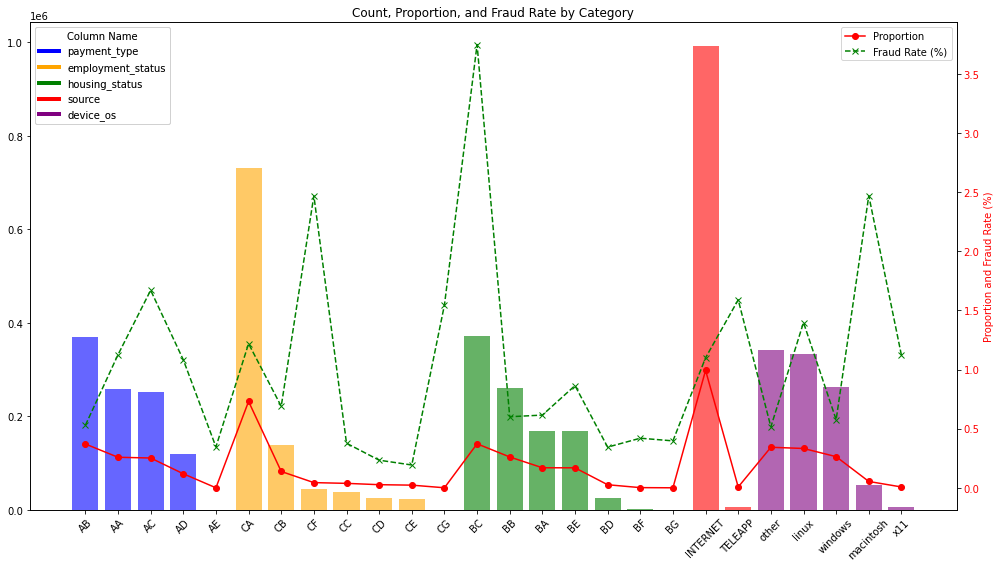
\includegraphics[width=\textwidth]{Count_Proportion_and_Fraud_Rate_by_Category.png}
    \caption{Count, Proportion, and Fraud Rate by Category and Column Name}
    \label{fig:count_proportion_fraud_rate}
\end{figure}

Figure \ref{fig:count_proportion_fraud_rate} presents the count (bars), proportion (red line), and fraud rate (green dashed line) for various categories within the columns: \textit{payment\_type}, \textit{employment\_status}, \textit{housing\_status}, \textit{source}, and \textit{device\_os}. Each bar color denotes a different column name.

The bars depict the number of occurrences for each category within their respective columns. Categories with the highest counts are seen across \textit{payment\_type}, \textit{employment\_status}, \textit{housing\_status}, \textit{source}, and \textit{device\_os}. The red line represents the proportion of occurrences for each category relative to the total. Categories such as INTERNET (from \textit{source}) and CA (from \textit{housing\_status}) have high proportions, indicating they constitute a significant portion of the data. The green dashed line with 'x' markers indicates the fraud rate for each category. Categories like BC (from \textit{payment\_type}) and macintosh (from \textit{device\_os}) exhibit higher fraud rates, suggesting a greater likelihood of fraudulent transactions within these categories.

High count and proportion categories dominate the dataset and require detailed analysis to understand their impact on overall fraud rates. High fraud rate categories indicate areas where fraud is more prevalent, necessitating targeted fraud prevention measures.

\section{Fraud Status and Distribution by Customer Age}

\begin{figure}[h]
    \centering
    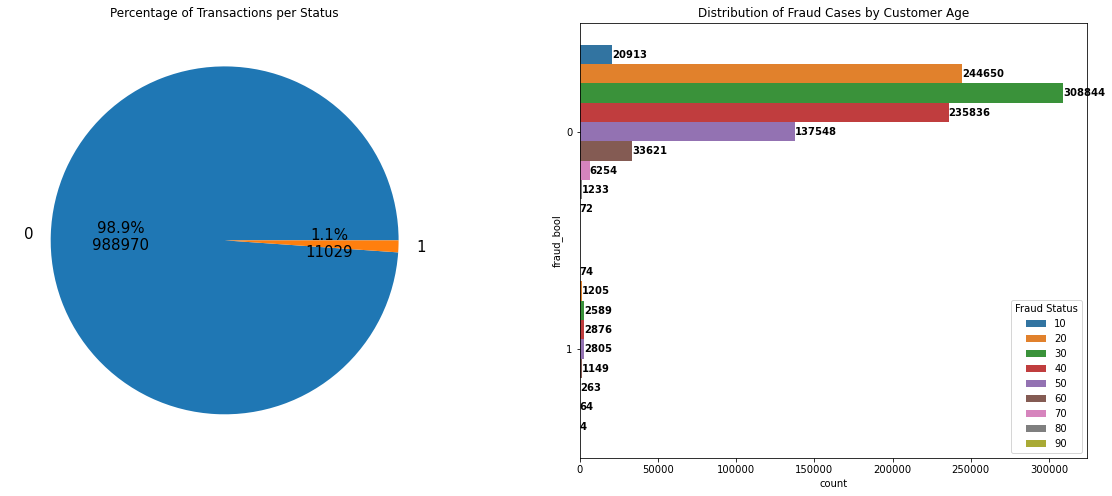
\includegraphics[width=\textwidth]{Distribution_of_Fraud_Cases.png}
    \caption{Fraud Status and Distribution of Fraud Cases by Customer Age}
    \label{fig:fraud_status_distribution_age}
\end{figure}

Figure \ref{fig:fraud_status_distribution_age} includes a pie chart showing the percentage of transactions per status (fraudulent vs. non-fraudulent) on the left, and a bar plot showing the distribution of fraud cases by customer age on the right. Non-fraudulent transactions represent 98.9\% of the total, totaling 988,970 transactions. Fraudulent transactions represent 1.1% of the total, totaling 11,029 transactions. This demonstrates a highly imbalanced dataset, with a significantly higher number of non-fraudulent transactions.

The distribution of fraud cases by customer age shows that:

\begin{itemize}
    \item Ages 30-40 have the highest count of fraud cases at 30,844.
    \item Ages 40-50 have the next highest count at 24,465.
    \item Ages 20-30 have 23,583 fraud cases.
    \item Ages 50-60 have 13,754 fraud cases.
    \item Ages 60-70 have 3,362 fraud cases.
    \item Ages 10-20 have 2,091 fraud cases.
    \item Ages 70-80 have 1,233 fraud cases.
    \item Ages 80-90 have 72 fraud cases.
    \item Ages 90-100 have 4 fraud cases.
\end{itemize}

Fraud cases are most prevalent among customers aged 30-50, suggesting individuals within this age range are more likely to be involved in fraudulent activities. There is a noticeable decline in fraud cases for customers aged above 60, with very few cases in the 80-100 age range.

\section{Income Distribution and Fraud Correlation}

The median income for non-fraudulent transactions is approximately 0.60 (decile form), with an interquartile range (IQR) of approximately 0.40 to 0.80, and a range of 0.10 to 0.90. For fraudulent transactions, the median income is approximately 0.80 (decile form), with an IQR of approximately 0.70 to 0.85, and a range of 0.30 to 0.90, with a few outliers below 0.30.

Higher income correlation with fraud is indicated as the median income for fraudulent transactions is higher compared to non-fraudulent transactions, indicating a higher association of fraud with higher income levels. Less variability in fraudulent income is observed as the IQR for fraudulent transactions is narrower compared to non-fraudulent transactions, indicating less variability in income among the fraudulent cases.

\section{Fraud Rate by Payment Type}

Fraud rates by payment type show that:

\begin{itemize}
    \item MC has the highest fraud rate at approximately 1.6%.
    \item MS has the next highest fraud rate at around 1.2%.
    \item MO has a fraud rate close to 1.0%.
    \item ME has the lowest fraud rate at around 0.4%.
    \item MA has a fraud rate slightly above 0.5%.
\end{itemize}

MC has the highest fraud rate, indicating transactions using payment type MC are more susceptible to fraud, warranting further investigation. ME has the lowest fraud rate, suggesting it appears to be the most secure or least targeted by fraud.

\section{Fraud Rate by Employment Status}

Fraud rates by employment status show that:

\begin{itemize}
    \item GE has the highest fraud rate at approximately 2.5%.
    \item GF has the next highest fraud rate at around 2.0%.
    \item GJ has a fraud rate close to 1.5%.
    \item GA has a fraud rate around 1.0%.
    \item GD has a fraud rate close to 0.5%.
    \item GG has a fraud rate below 0.5%.
    \item GH has a fraud rate below 0.5%, but slightly higher than GG.
    \item GC has a fraud rate around 0.5%.
\end{itemize}

GE has the highest fraud rate, indicating individuals with employment status GE are more susceptible to fraud, necessitating further investigation. GF also shows a high fraud rate, requiring attention for individuals with employment status GF.

\section{Fraud Rate by Housing Status}

Fraud rates by housing status show that:

\begin{itemize}
    \item BA has the highest fraud rate at approximately 3.5%.
    \item BD has the next highest fraud rate at around 1.0%.
    \item BE, BF, and BG have fraud rates close to 0.5%.
    \item BB and BC have fraud rates around 0.8%.
    \item BH has a fraud rate below 0.5%, but slightly higher than BE, BF, and BG.
\end{itemize}

BA has the highest fraud rate, indicating individuals with housing status BA are significantly more susceptible to fraud, requiring further investigation. BD shows a moderate fraud rate, indicating individuals with housing status BD also have a relatively higher fraud rate.

\section{Fraud Rate by Source of Request}

\begin{figure}
    \centering
    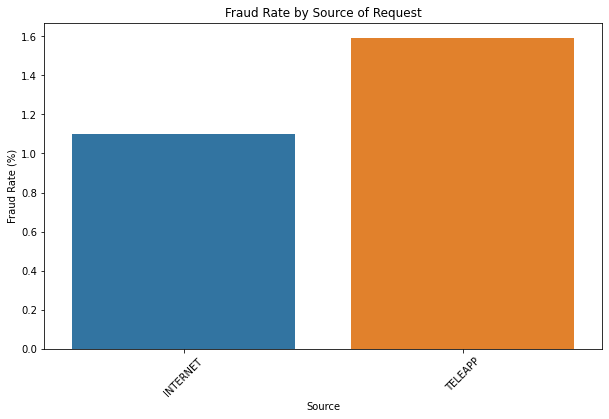
\includegraphics[width=\textwidth]{Fraud_Rate_by_Source_of_Request.png}
    \caption{Fraud Rate by Source of Request}
    \label{fig:fraud_rate_source_of_request}
\end{figure}

Figure \ref{fig:fraud_rate_source_of_request} illustrates the fraud rate (percentage) for each source of request. 

\begin{itemize}
    \item TELEAPP has the highest fraud rate at approximately 1.6%.
    \item INTERNET has a lower fraud rate at around 1.2%.
\end{itemize}

TELEAPP has a higher fraud rate, indicating requests from TELEAPP are more susceptible to fraud compared to INTERNET, warranting further investigation. INTERNET shows a lower fraud rate, indicating it is significant but lower than TELEAPP.

\section{Fraud Rate by Device OS}

Fraud rates by device OS show that:

\begin{itemize}
    \item Windows has the highest fraud rate at approximately 2.5%.
    \item Macintosh has the next highest fraud rate at around 1.5%.
    \item iOS has a fraud rate close to 1.0%.
    \item Other has a fraud rate around 0.7%.
    \item Linux has the lowest fraud rate at around 0.5%.
\end{itemize}

Windows has the highest fraud rate, indicating devices running Windows OS are more susceptible to fraud, requiring further investigation. Macintosh also shows a relatively high fraud rate, suggesting attention should be given to devices running Macintosh OS.

This exploratory data analysis provides valuable insights into the distribution and patterns of fraud within the dataset, guiding further analysis and model development for effective fraud detection.









\chapter{Results and Discussion}





\chapter{Conclusion}



\bibliographystyle{apalike}
\bibliography{references}


\end{document}
